\section{Comparison data simulation}
Now that  we have a  good simulation of  each step of  the electronics
chain, we  want to test  the simulation with  the data. One way  to do
that is  by looking at  the fluctuations of  the radio signal  that we
measure in the recorded events. So we will carry out a full simulation
and compare the distribution of the  radio signal in ADC units. \\ The
fluctuations of  the radio  signal depend on  one other input  that we
haven't looked  at yet: the LNB bandwidth.  The formula is
given by:
\begin{equation}
  \rm \frac{\sigma}{\mu} \propto \frac{1}{\sqrt{\Delta B \cdot \tau}}
  \label{eq:sigmamuprop}
\end{equation}

where  $\rm \Delta  B$  is the  bandwidth  and $\rm  \tau$  is a  time
constant  of the  detector.  We  will try  to  understand better  this
formula and add the proportionalty coefficients in the last section.
\subsection{Bandwidth}
First   let's   see   why   what   we   want   to   include   in   the
equation~\ref{eq:sigmamuprop} is  the bandwidth defined  with the gain
(and  not the  effective area  for instance).  What comes  out  of the
antenna + LNB is:
\begin{equation}
   \rm P(\nu) = \frac{1}{2}\int_\Omega F(\nu) A_{eff}(\nu) G_{LNB}(\nu)d\Omega
\end{equation}
with 
\begin{equation}
  \rm F(\nu) = \frac{2k_B T \nu^2}{c^2}
\end{equation}
and 

\begin{equation}
  \rm A_{eff}(\nu) = \frac{ G_{ant}(\nu)c^2 }{4\pi \nu^2 }
\end{equation}


So the  $\rm \nu^2$ cancels  out and we  have only:
\begin{equation}
   \rm P(\nu) = \frac{1}{4\pi}\int_\Omega k_B T G_{ant}(\nu) G_{LNB}(\nu) d\Omega= k_B T_{ant} G_{LNB}(\nu)
\end{equation}
Up  to now  we were  considering a  nominal bandwidth,  something like
800~MHz because the  C-band is defined between 3.4  and 4.2~GHz.  This
assumes that the gain is flat in frequency. But we can consider a more
precise definition:
\begin{equation}
   \rm \Delta B = \frac{1}{G_{max}} \int G(\nu) \cdot d\nu
   \label{eq:eqdeltab}
\end{equation}
We have access to the measured bandwidth for the two types of antennas:
\begin{itemize}
\item for EASIER antennas (DMX and GI301):spectrum measurement (in the field or at room temperature)
\item for GIGADuck antenna (AINFO) : IMEP measurement of the LNB gain
\end{itemize}

\begin{figure}[!ht]
  \centering
  \hspace*{-3ex}
  \subfigure{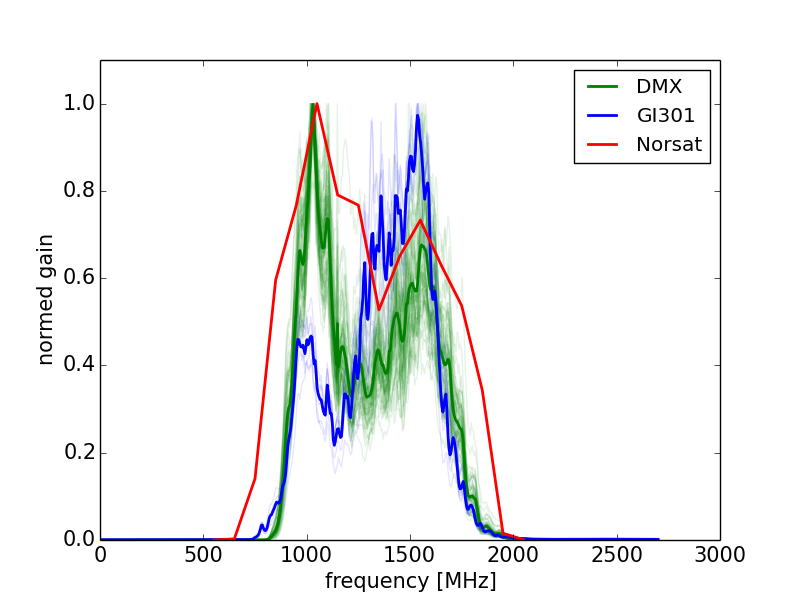
\includegraphics[width=0.60\linewidth]{spectra3.png}}
  \caption{gain spectra for the three types of LNB in the C-band. The blue one is a average of the light blue ones.}
  \label{fig:spectra}
\end{figure}

\begin{table}[h!]
  \centering
  \caption{bandwidths}
  \label{tab:tabdeltab}
  \begin{tabular}{|c||c|c|c|}
    \hline
    antenna type & GI301  & DMX & Norsat \\
    \hline
    bandwidht & 437 $\rm \pm 30$& 445 $\rm \pm$ 56 & 750.1\\
    \hline
  \end{tabular}
\end{table}




\textbf{remark:  if the  VSWR of  the  antenna is  large, meaning  the
  bandwidth is limited  by the antenna and not  the amplifier, then we
  have  to account  for the  then  antenna VSWR  (or equivalently  the
  transmission coefficient).}\\  The spectra of  the different antenna
are  given in  figure~\ref{fig:spectra},  the corresponding  bandwidth
computed   according  equation~\ref{eq:eqdeltab}   are   given  in   the
tab~\ref{tab:tabdeltab}.

\subsection{full simulation and comparison with data}
\subsubsection{data}
To measure the RMS of the  detectors installed in the field, we select
events with EASIER  station hit and just histogram  the radio waveform
in ADC (after  removing the baseline). We have  picked arbitrarely the
month  of  April 2015  (it  is  the period  when  all  the arrays  are
present).  We  show as an example  3 waveforms, one for  each array of
the C-band  in the  figure~\ref{fig:datatrace} (left) and  the average
RMS  is shown  for all  the stations  during the  chosen month  in the
figure~\ref{fig:datatrace} (right). Most of the EASIER61 detector have
their RMS around  50 and some of  them to be off (close  to zero). For
the EASIER7  the RMS is lower  because the capacitor  is present after
the power  detector. Finally all  the GIGADUCK detectors  (except one)
have their RMS between 47 and 50.

\begin{figure}[!ht]
  \centering
  \hspace*{-3ex}
  \subfigure{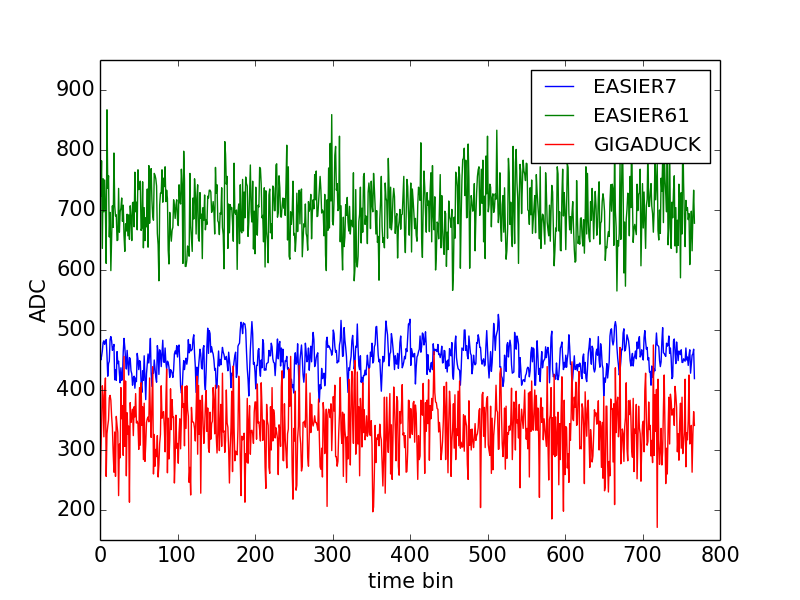
\includegraphics[width=0.49\linewidth]{datatrace.png}}
  \subfigure{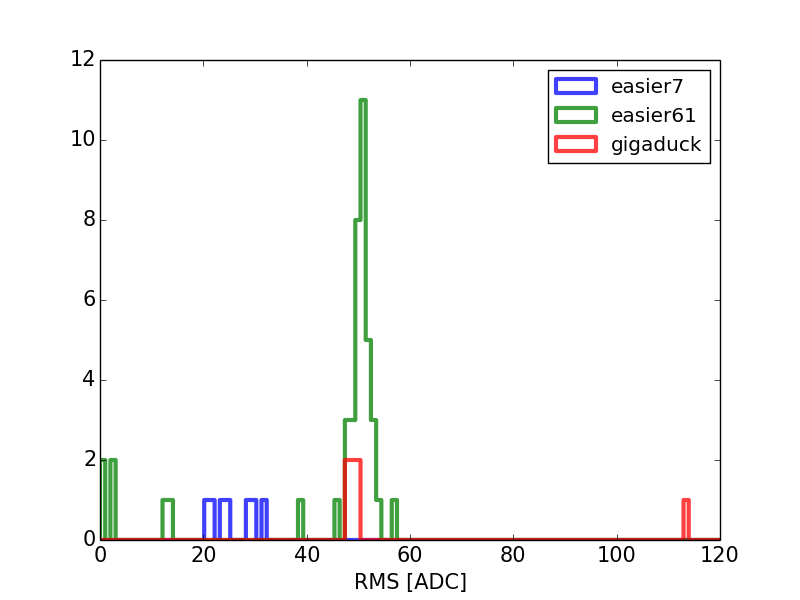
\includegraphics[width=0.49\linewidth]{datarmsdist.png}}
  \caption{example of trace from each detector in the C-band. right: distribution of the average RMS of all detectors}
  \label{fig:datatrace}
\end{figure}

\begin{figure}[!ht]
  \centering
  \hspace*{-3ex}
  \subfigure{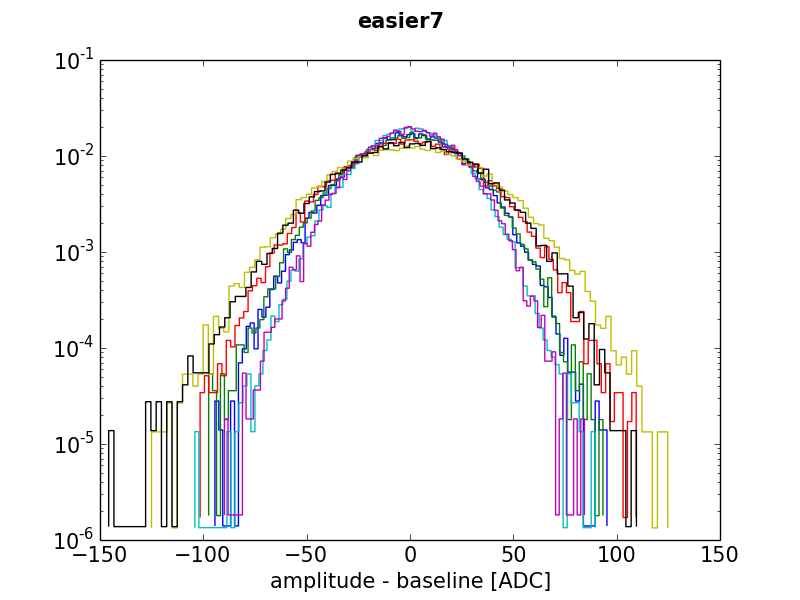
\includegraphics[width=0.32\linewidth]{disteasier7.png}}
  \subfigure{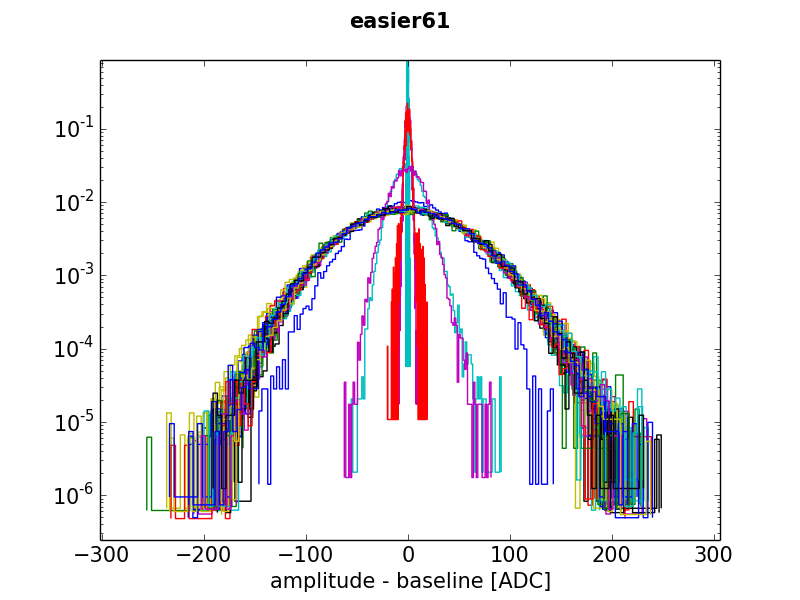
\includegraphics[width=0.32\linewidth]{disteasier47.png}}
  \subfigure{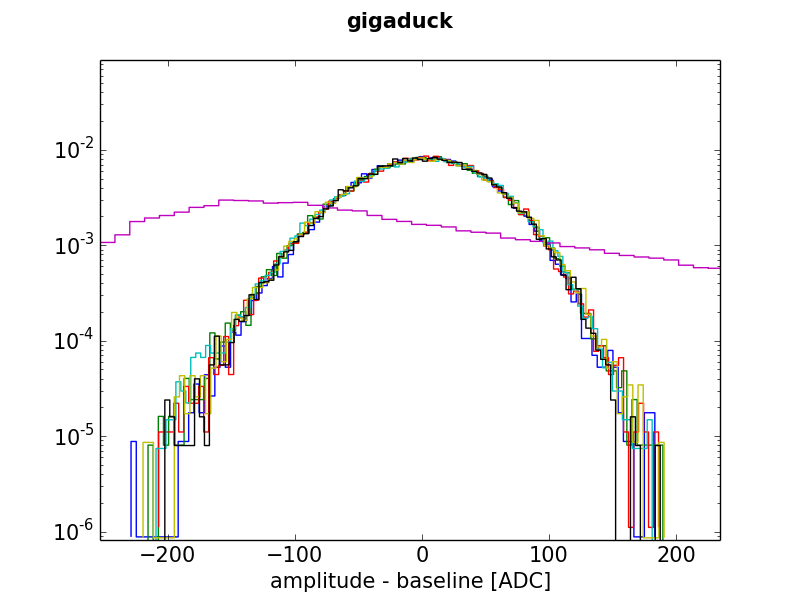
\includegraphics[width=0.32\linewidth]{distgigaduck.png}}
  \caption{example of trace from each detector in the C-band. right: distribution of the average RMS of all detectors}
  \label{fig:datatrace}
\end{figure}

\subsubsection{simulation}
Now we can  produce HF waveforms from the  measured spectra, then make
the  waveform go through  the electronics  simulation we  described in
section 1. Figure~\ref{fig:compdist}  shows the measured and simulated
distribution     of      amplitude     in     ADC      counts,     and
figure~\ref{fig:compmeanrms} compares the  average RMS (we removed the
bad stations).


%% \begin{figure}[!ht]
%%   \centering
%%   \hspace*{-3ex}
%%   \subfigure{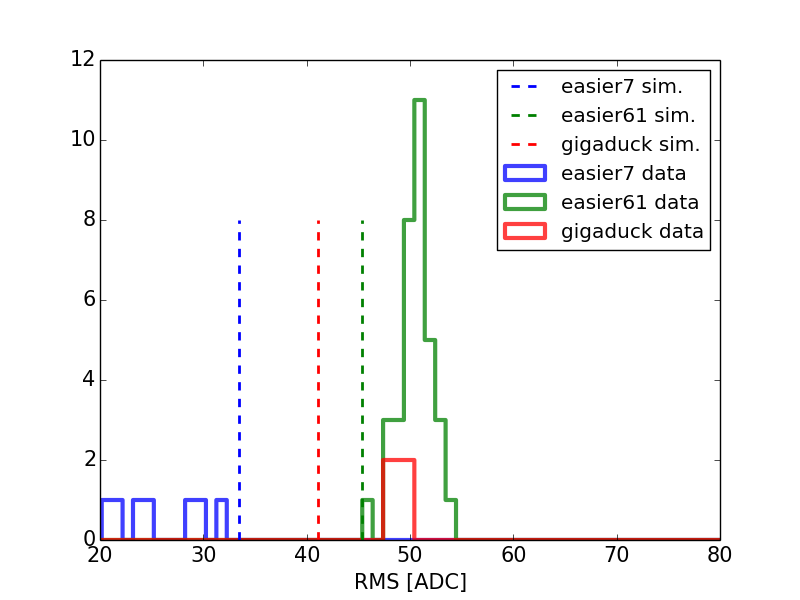
\includegraphics[width=0.49\linewidth]{datasimrmsdist.png}}
%%   \caption{example of trace from each detector in the C-band. right: distribution of the average RMS of all detectors}
%%   \label{fig:datatrace}
%% \end{figure}

\begin{figure}[!ht]
  \centering
  \hspace*{-3ex}
  \subfigure{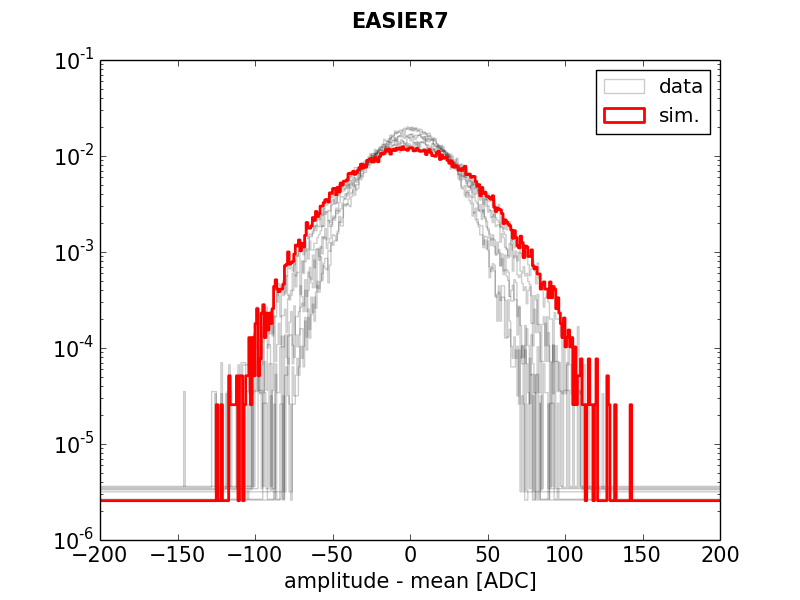
\includegraphics[width=0.32\linewidth]{distdatasimEA7.png}}
  \subfigure{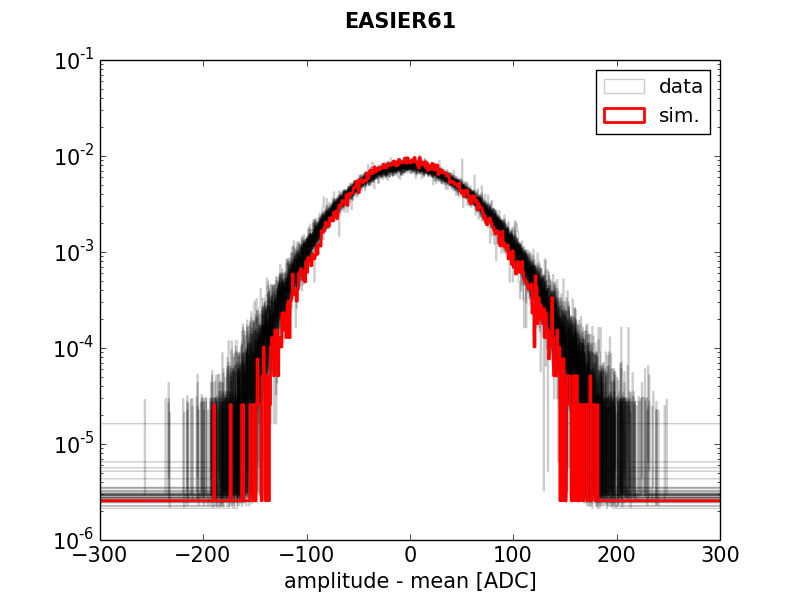
\includegraphics[width=0.32\linewidth]{distdatasimEA61.png}}
  \subfigure{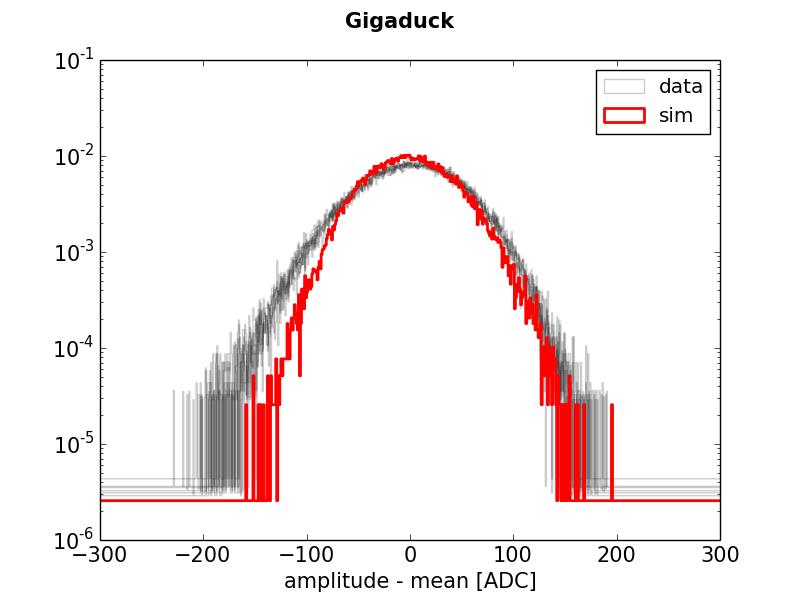
\includegraphics[width=0.32\linewidth]{distdatasimGD.png}}
  \caption{comparison of the measured distribution of amplitude and the simulated one.}
  \label{fig:datatrace}
\end{figure}

\begin{figure}[!ht]
  \centering
  \hspace*{-3ex}
  \subfigure{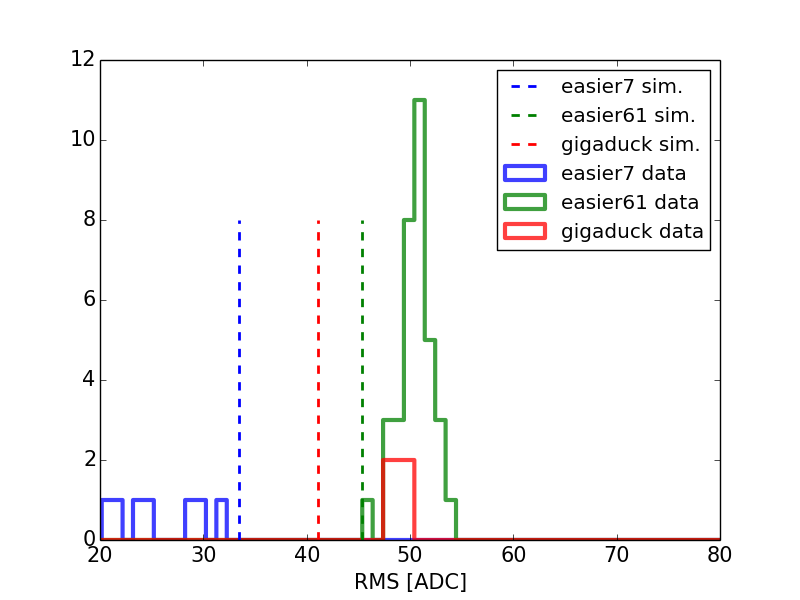
\includegraphics[width=0.60\linewidth]{datasimrmsdist.png}}
  \caption{comparison of the measured distribution of amplitude and the simulated one.}
  \label{fig:datatrace}
\end{figure}

At the end  the average value of the RMS are  smaller for EASIER61 and
GIGADUCK and larger for EASIER7. I  think that the reason might be the
parameters found in  section 1. When I fit the  time constant I obtain
at  the  same time  the  characteristic of  the  power  detector (V  =
f(power)). When we look  at the value a and b obtain  for the two case
we see that they are different and the final fluctuation are sensitive
to  the parameter  a  (the slope).   Especially  we see  that for  the
capacitor case the  slope is larger than the  no capacitor case, which
goes in the  same trend as the  discrepancy in the RMS (I  mean if the
value of a was taken as the  mean of the two value we would reduce the
discrepancies of both cases.) Another possibility is that the response
is a  little different for the noise  part and the signal  part. In my
thesis I had found a difference  in the fit results for the noise part
and the signal part. 
 


\begin{figure}[!ht]
  \centering
  \hspace*{-3ex}
  \subfigure{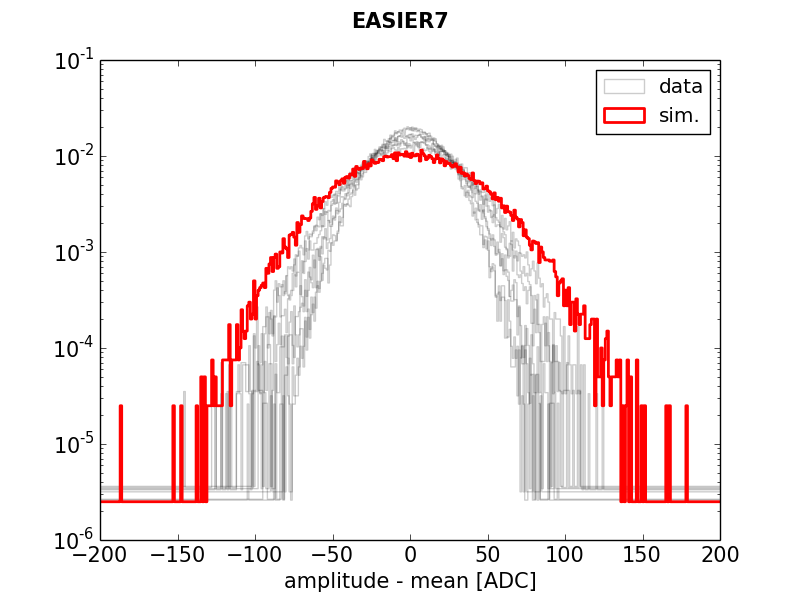
\includegraphics[width=0.32\linewidth]{m2_distdatasimEA7.png}}
  \subfigure{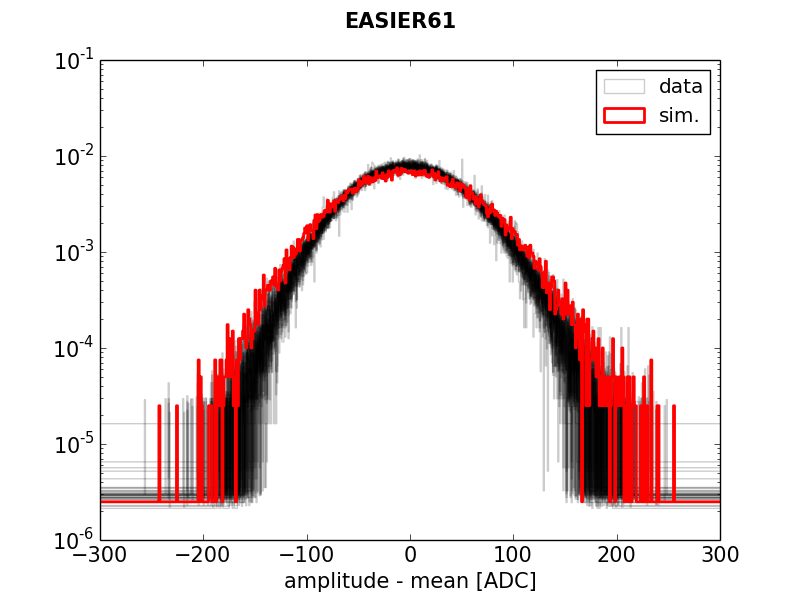
\includegraphics[width=0.32\linewidth]{m2_distdatasimEA61.png}}
  \subfigure{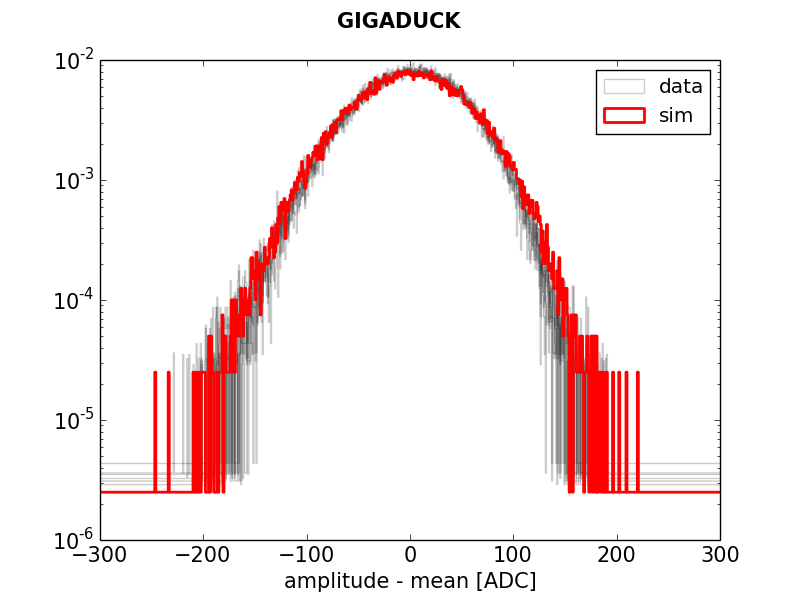
\includegraphics[width=0.32\linewidth]{m2_distdatasimGD.png}}
  \caption{comparison of the measured distribution of amplitude and the simulated one.}
  \label{fig:m2_distdata}
\end{figure}

\begin{figure}[!ht]
  \centering
  \hspace*{-3ex}
  \subfigure{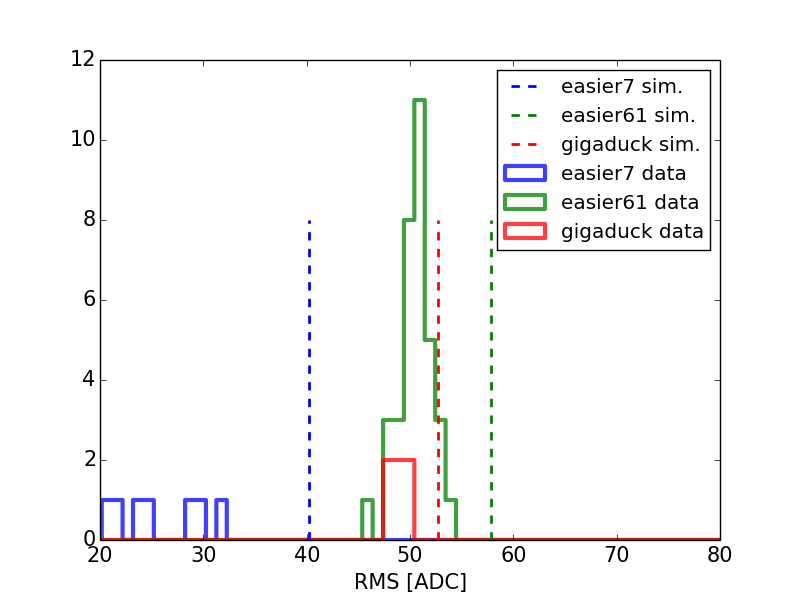
\includegraphics[width=0.60\linewidth]{m2_datasimrmsdist.png}}
  \caption{comparison of the measured distribution of amplitude and the simulated one.}
  \label{fig:m2_comprms}
\end{figure}


\begin{figure}[!ht]
  \centering
  \hspace*{-3ex}
  \subfigure{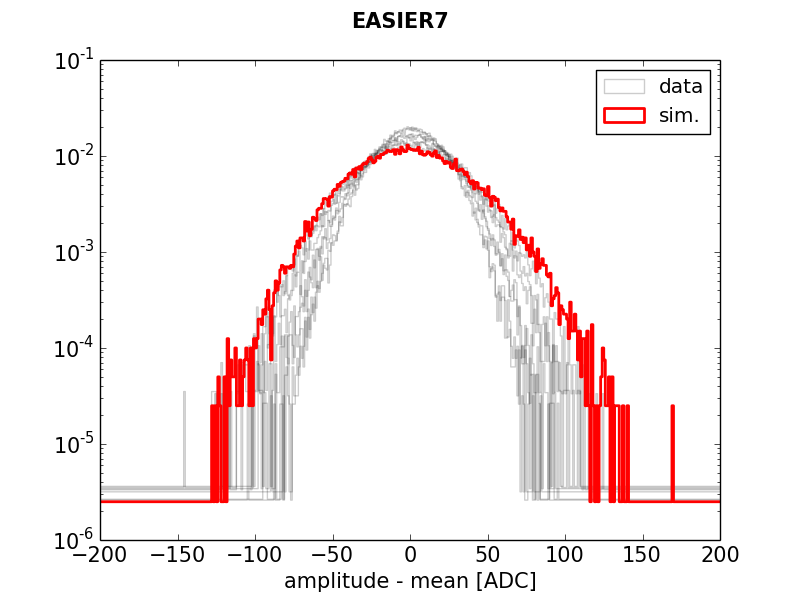
\includegraphics[width=0.32\linewidth]{m3_distdatasimEA7.png}}
  \subfigure{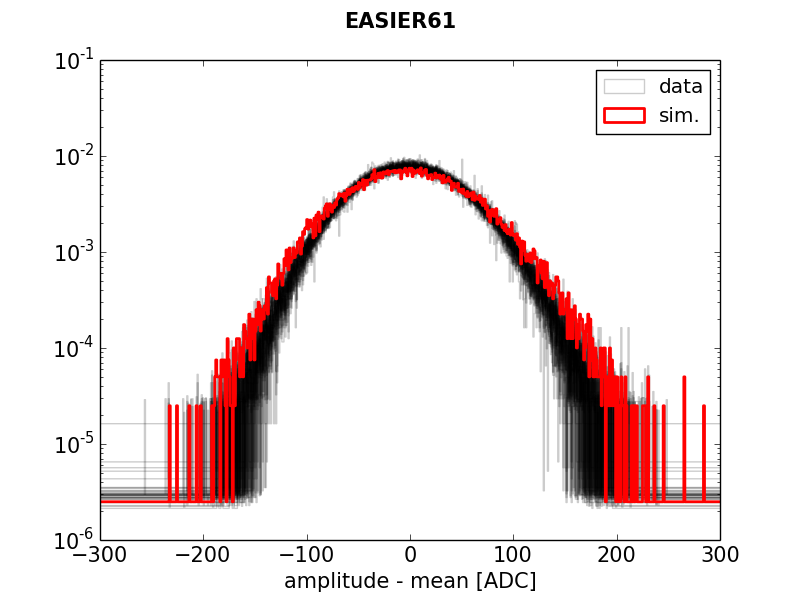
\includegraphics[width=0.32\linewidth]{m3_distdatasimEA61.png}}
  \subfigure{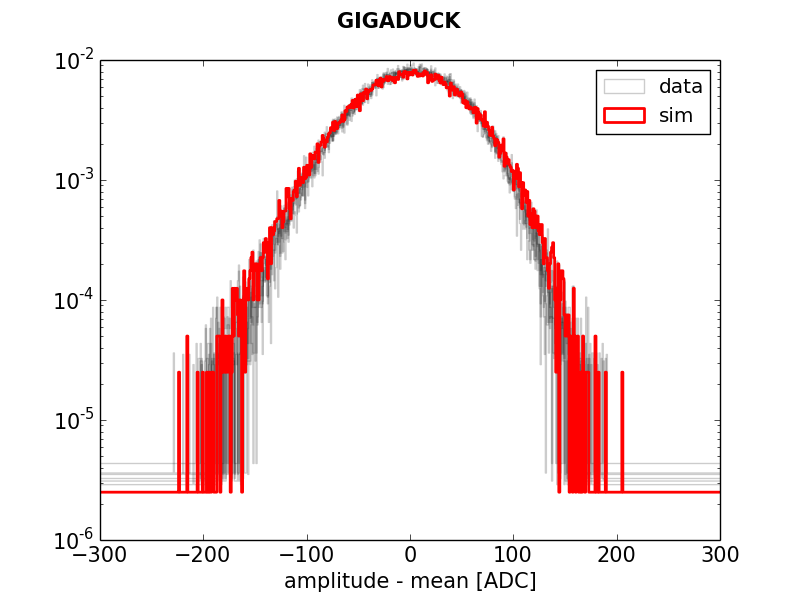
\includegraphics[width=0.32\linewidth]{m3_distdatasimGD.png}}
  \caption{results for third method}
  \label{fig:m3_distdata}
\end{figure}

\begin{figure}[!ht]
  \centering
  \hspace*{-3ex}
  \subfigure{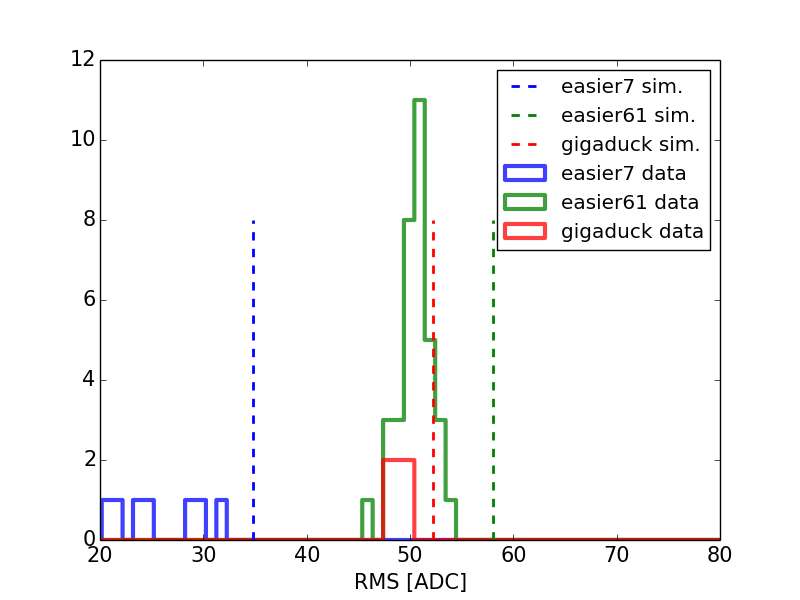
\includegraphics[width=0.60\linewidth]{m3_datasimrmsdist.png}}
  \caption{results for third method}
  \label{fig:m3_comprms}
\end{figure}




